\subsection{Moran's I as a measure for spatial (in)homogeneity between
oscillating cells}

In mammals, the SCN seems to play the central role in coordinating the
circadian rhythms across the whole
organism~\cite{reppert2002coordination}. The SCN is a densely packed
brain region containing dozens of thousands of rhythmic neurons and
can be anatomically classified in several regions, depending on what
neurotransmitter the underlying neurons can secret and react to. The
dorsal and ventral parts of the SCN represents the most obviously
different parts of the whole organ~\cite{yamaguchi2003synchronization}
and show quite different rhythmical behaviour. In this subproject, we
aimed at quantifying the spatial inhomogeneities across SCN slices in
terms of their synchronization properties.

The standard way to quantify the degree of synchronization in an
ensemble of oscillators has traditionally been the Kuramoto order
parameter $R$~\cite{kuramoto2012chemical}. The idea behind can be
visualized by placing each of the interacting oscillators on a unit
circle according to the oscillator's instantaneous phase and
calculating the centroid of resulting distribution of oscillators. The
absolute value of $R$, i.e. the distance of the centroid from the
origin, would then show the degree of instantaneous synchronization.
If, for instance, all oscillators are (nearly) uniformly distributed
along the unit circle, their centroid would be very close to origin
and $R$ would be close to zero. On contrary, if most of the
oscillators are grouped around a preferred phase, the centroid would
be close to that point and its distance from the origin (the absolute
value of $R$) would be close to one.

\begin{figure}
\begin{center}
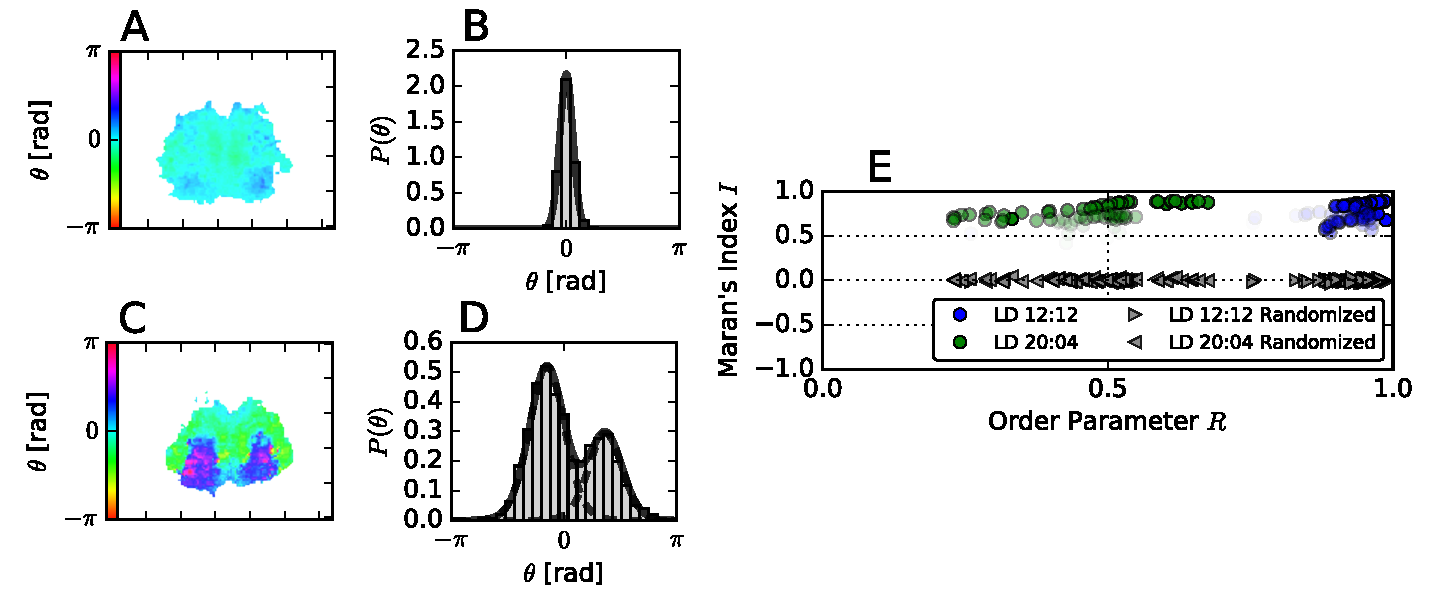
\includegraphics[width=\linewidth]{figures/mi/mi.pdf}
\end{center}
\caption{
  {\bf (A)} and {\bf (C)} Colour-coded distribution of oscillation
  phases of neurons across an SCN slice under equinox and long-day
  conditions, respectively.
  {\bf (B)} and {\bf (D)} The corresponding distributions of phases.
  {\bf (E)} Time traces in the coordinate plane of Kuramoto's order
  parameter $R$ and Moran's I.
\label{fig::mi}
}
\end{figure}

This approach, however, assumes no special arrangement between the
oscillating units, such as, for example, their ordering in space
relatively to each other. Looking for a better way to measure such
spatial aspect of synchronization across neurons, Dr Christoph Schmal
stumbled upon the so-called Moran's I statistics, which has been
widely used in geographical and sociological sciences for quantifying
the spatial correlation in units with a certain arrangement in
space~\cite{moran1950notes}. Moran's I takes into account the
arrangement of units in space by calculating the correlation between
the units weighted by the distance between them. So, for example, a
black and white chess board would corresponding to a Moran's I value
of $-1$, reflecting the largest possible anti-correlation between
neighbouring units and a uniform homogeneous state would correspond to
the Moran's I value of 1 (the largest possible value). Moran's I
turned out to complement the traditional Kuramoto's order parameter
$R$ in a most insightful way when analyzing the rhythmicity of neurons
in SCN slices~\cite{schmal2017moran}. Figure~\ref{fig::mi} from that
paper shows two examples of phase distribution across SCN slices (see
(A) and (B) for colour-coded representations and (B) and (D) for the
probability distribution of phases).

When plotting the values of Moran's I vs Kuramoto's order parameter
$R$ (Figure~\ref{fig::mi} (E)), we have found scenarios with both
statistics giving complementary results. It is, for example, possible
that Moran's I remains close to zero, whereas the order parameter $R$
is non-zero. This situation would emerge when all neurons have phases
close to each other but the spatial correlation between neighbouring
neurons is absent. The opposite situation with relatively low values
of Kuramoto's order parameter $R$ and Moran's I close to one arises
when the spread of phases between the oscillators is large, but most
neighbours are relatively strongly correlated (green dots in
Figure~\ref{fig::mi} (E)). The influence of the photoperiod on the
observed interplay beween $R$ and Moran's I certainly deserves further
investigation, also in the light of the above discussion of the role
of photoperiod in entrainment phase.
